\section{Имплементация кадрового графа}
Концептуально работу с кадровыми графами можно разбить на три этапа - \textit{декларация}, \textit{компиляция} и \textit{исполнение}.

На этапе декларации разработчик определяет структуру графа, описывая узлы и зависимости между ними. Важно на этом этапе чётко определить зависимости между задачами, чтобы гарантировать правильную последовательность их выполнения.

Этап декларации — это этап, на котором определяется структура кадрового графа. В ходе этого этапа разработчики декларируют задачи, ресурсы и их зависимости. Это включает в себя указание, какие ресурсы читаются или записываются каждой задачей рендеринга. Четко определяя эти зависимости, кадровый граф гарантирует, что ресурсы не будут одновременно использоваться конфликтующими способами, что могло бы привести к артефактам рендеринга или сбоям. Кроме того, этап декларации помогает организовать конвейер рендеринга модульным образом, что облегчает его управление и расширение.

После того как кадровый граф задекларирован, он переходит на этап компиляции. На этом этапе кадровый граф анализируется для определения оптимального порядка выполнения задач. Это включает в себя разрешение зависимостей, чтобы каждая задача выполнялась только после того, как все ее входные ресурсы были созданы предыдущими задачами. Этап компиляции также включает выделение ресурсов, где система решает, как эффективно использовать доступную память. Это может включать повторное использование ресурсов, где это возможно, для минимизации использования памяти.

Заключительный этап — это исполнение, на котором скомпилированный кадровый граф используется для управления процессом рендеринга. В ходе исполнения задачи выполняются в порядке, определенном на этапе компиляции, обеспечивая соблюдение всех зависимостей. Этот этап включает в себя выдачу соответствующих команд отрисовки и вычислительных задач на GPU, управление выставлением ресурсов и обеспечение синхронизации между различными задачами.

\subsection{Описание программного интерфейса}
Прежде всего рассмотрим разработанный программный интерфейс как самого кадрового графа, так и RHI, чтобы иметь общую картину архитектуры и целей последующей имплементации.

\subsubsection{Внедрение в Render Hardware Interface}
Ключевая идея в дизайне RHI данной работы -- не предоставлять доступ к созданию и отправке на исполнение командных буферов. Это заставляет выражать всю вычислительную работу с GPU посредством кадровых графов. Данный подход позволяет более точечно оптимизировать каждую реализацию RHI с учетом особенностей конкретного графического API и аппаратного обеспечения, вместо того, чтобы пытаться обобщить работу с командными буферами между API. Помимо этого, разработчикам, использующим RHI для написания более высокоуровневых модулей, будет проще и удобнее выражать свои идеи через граф, декомпозируя сложные алгоритмы на небольшие задачи, имея глобальную визуализацию рендеринга и не погружаясь в низкоуровневые детали работы с командами в графических интерфейсах.

\begin{figure}[h]
    \centering
    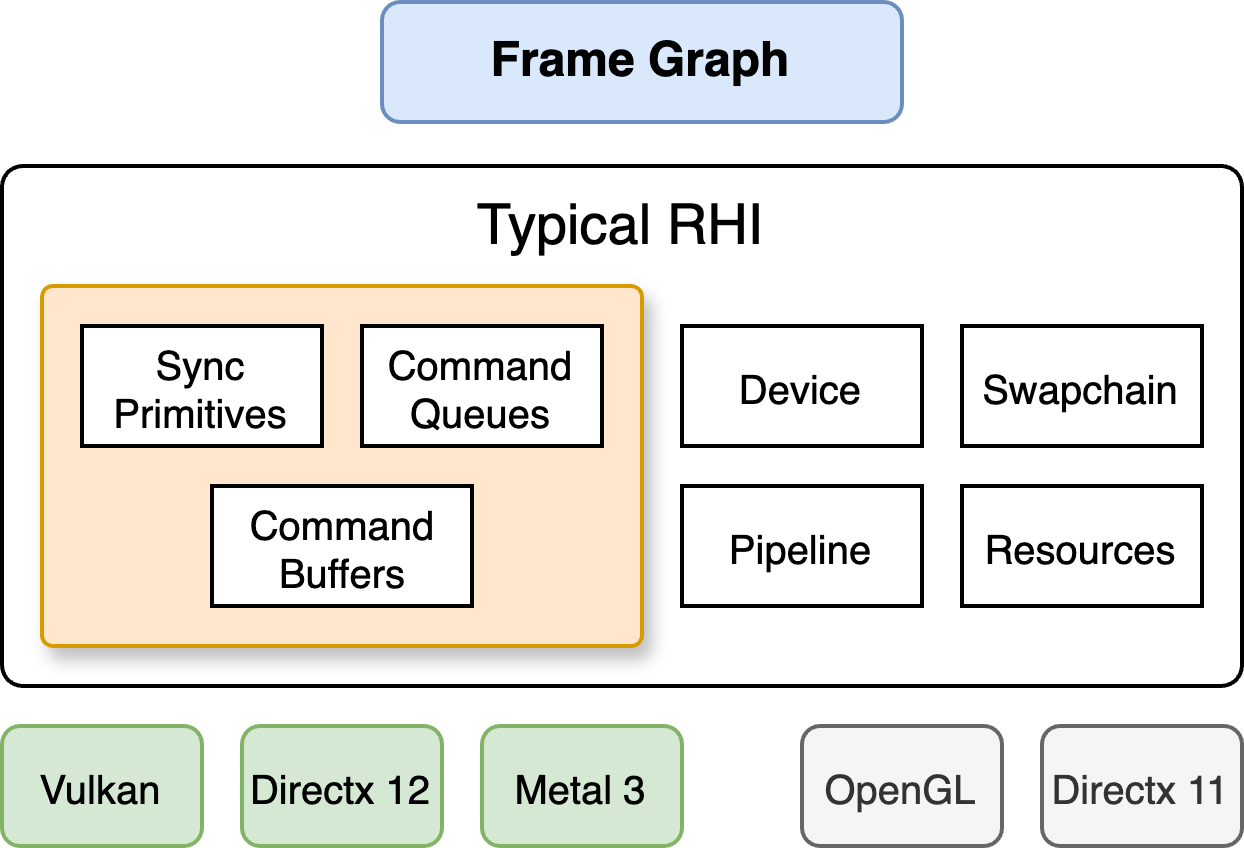
\includegraphics[scale=0.175]{rhi/typical_rhi_diagram.png}
    \hfill
    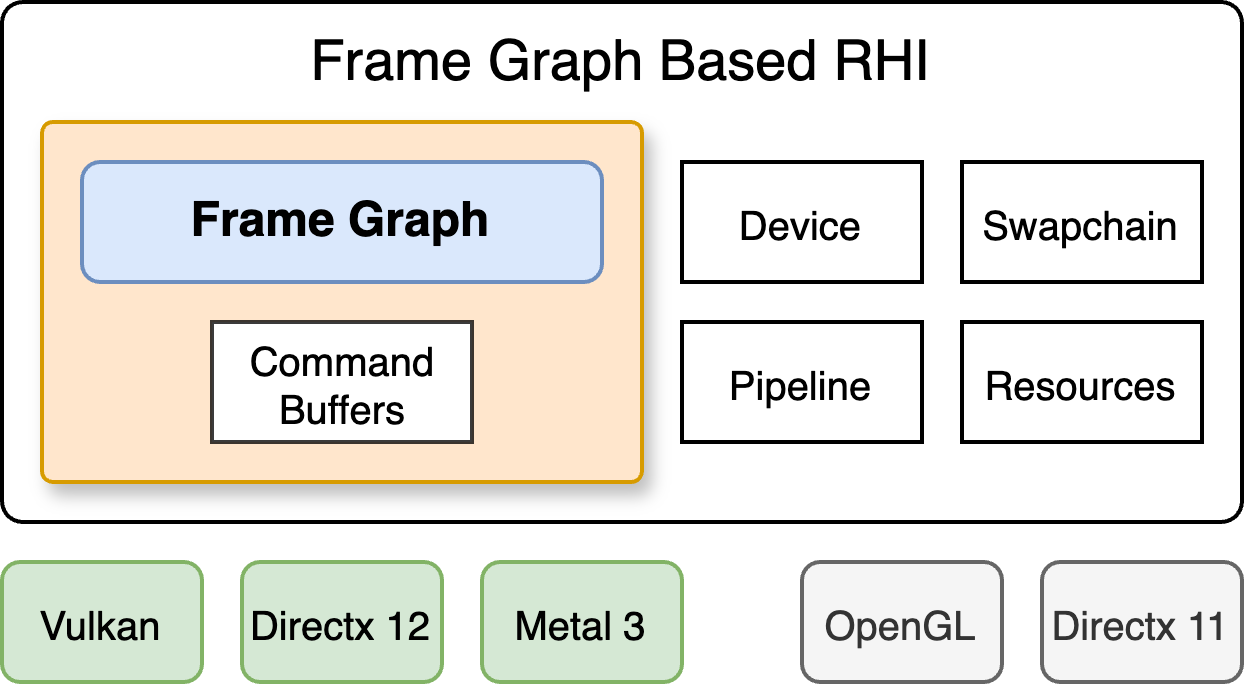
\includegraphics[scale=0.175]{rhi/frame_graph_based_rhi_diagram.png}
    \caption{Сравнение типичного дизайна RHI (слева) и дизайна, предложенного в данной работе, внедряющего кадровый граф напрямую в RHI (справа).}
    \label{fig:rhi_design_comparison}
\end{figure}

На рисунке \ref{fig:rhi_design_comparison} представлено сравнение типичной структуры RHI и структуры, предложенной в данной работе. Как видно из рисунка, получилось избавиться от абстракции примитивов синхронизации и командных очередей. Не смотря на то, что командные буферы остались как класс в RHI, методы их создания и отправки на исполнения не предоставляются, всем этим занимается кадровый граф. Как уже было сказано, данный подход дает полную свободу при имплементации RHI, поскольку нет необходимости в попытках обобщить интерфейсы всех графических API, как это сделано в типичном дизайне.

\subsubsection{Декларация кадрового графа}
На этапе декларации графа задаются вершины, а также ресурсы, которые будут использоваться. Вершина графа может быть одного из трех типов -- \textit{graphics}, \textit{compute} или же \textit{transfer}. Ресурсы, в свою очередь, могут быть либо вспомогательными, либо импортированными. Первыми владеет и управляет кадрового граф, вторыми же он только пользуется. Каждому использованию ресурса присваивается некоторое уникальное целое число -- \textit{версия}. Пример декларации графической вершины представлен в листинге \ref{lst:render_graph_declaration}. Компиляцией занимается конкретная имплементация RHI, на этом этапе создаются все необходимые объекты для исполнения кадрового графа. На этапе исполнения конкретная имплементация проходит в нужном порядке по вершинам, вызывает задачу, ассоциированную с данной вершиной на этапе декларации и занимается автоматически расстановкой синхронизации, контекста, отправляет работу на графический процессор и т.д.

\begin{minipage}[h]{0.95\textwidth}
\centering
\begin{cpp}[language=C++, caption={Пример декларации графической вершины графа.}, label={lst:render_graph_declaration}]
auto rg_color = builder.DeclareImportTexture(...);
auto rg_depth = builder.DeclareTransientTexture(...);

builder.BeginRenderPass("Forward Pass");
builder.AddColorTarget(rg_color, ...);
builder.SetDepthStencil(rg_depth, ...);
builder.SetJob([](CommandBuffer& cmds) {
    ...
});
builder.EndRenderPass();
\end{cpp}
\end{minipage}

Часто бывает необходимо декларировать временные ресурсы, чьи параметры зависят от других ресурсов. Например, это может быть буфер глубины, ведь его размер должен совпадать с размерами окна, т.е. главного рендер таргета. В связи с этим функции декларации временных ресурсов принимают структуру, похожую на обычную спецификацию ресурса, но у которой некоторые поля (такие как напр. размер) могут помимо точного значения принимать версию ресурса кадрового графа, показывая зависимость. Пример такой декларации показан в \ref{lst:render_graph_dependent_texture_info}.

\begin{minipage}[h]{0.95\textwidth}
\centering
\begin{cpp}[language=C++, caption={Пример декларации зависимых временных ресурсов.}, label={lst:render_graph_dependent_texture_info}]
auto rg_color = builder.DeclareImportTexture(...);

rhi::FrameGraph::DependentTextureInfo depth_info{};
depth_info.extent.SetDependency(rg_color);
depth_info.format = rhi::Format::D32_SFLOAT;
depth_info.type   = rhi::TextureType::Texture2D;
depth_info.usage  = rhi::DeviceResourceState::DepthStencilTarget;
...
depth_info.name   = "Depth buffer";

auto rg_depth = builder.DeclareTransientTexture(depth_info);
\end{cpp}
\end{minipage}

\subsection{Алгоритм компиляции}
\subsubsection{Топологическая сортировка}
\begin{wrapfigure}{R}{0.305\textwidth}
    \centering
    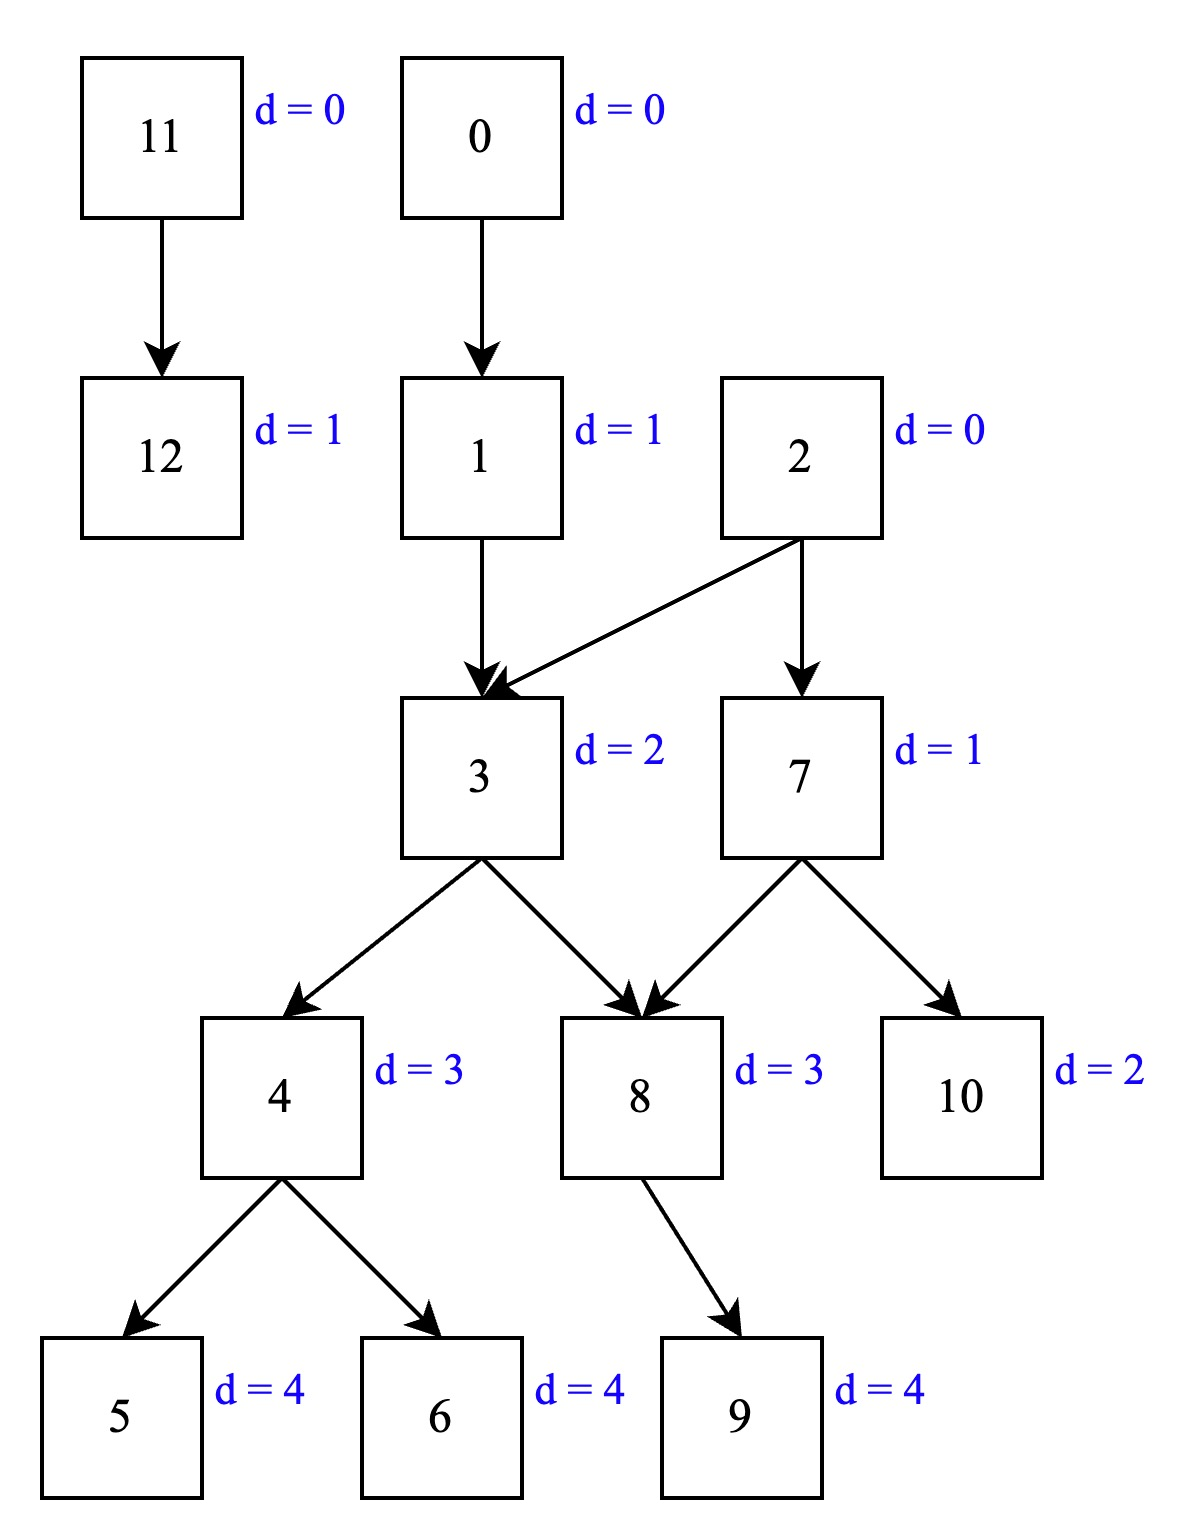
\includegraphics[scale=0.115]{rhi/render_graph/topological_sort_graph.jpeg}
    \caption{Граф зависимостей.}
    \label{fig:render_graph_topological_sort_graph}
\end{wrapfigure}

Первая часть компиляции кадрового графа -- топологическая сортировка, она является универсальной для всех имплементаций. Предположим у нас есть $V$ вершин графа и уже расставленные ребра между ними, где ребро $(u, v)$, означает что вершина $v$ должна исполняться после $u$. В дальнейшем нам также понадобится глубина (или по-другому \textit{dependency level}) каждой вершины, обозначим ее $d(u)$. Глубина вершины помогает определить какие вершины потенциально могут исполняться параллельно. Она определяется как минимальная из всех возможных реберная длина пути от некоторой вершины $s$, в которую не ведут никакие ребра. За один обход в глубину графа мы сможем получить как глубины всех вершин, так и некоторую топологическую сортировку. Однако произвольная топологическая сортировка нам не подойдет. Необходимо, чтобы в получившейся сортировке глубины вершин монотонно не убывали. Для этого необходима дополнительная сортировка массива. Результат данной части алгоритма для графа \ref{fig:render_graph_topological_sort_graph} проиллюстрирован на рисунке \ref{fig:render_graph_topological_sort_arrays}. Данная часть алгоритма позволяет преждевременно обнаружить циклические зависимости и обеспечивает корректный порядок всех задач в графе. Кроме того, монотонное неубывание глубин помогает в дальнейшем распределении ресурсов и синхронизации выполнения.

\begin{figure}[h]
    \centering
    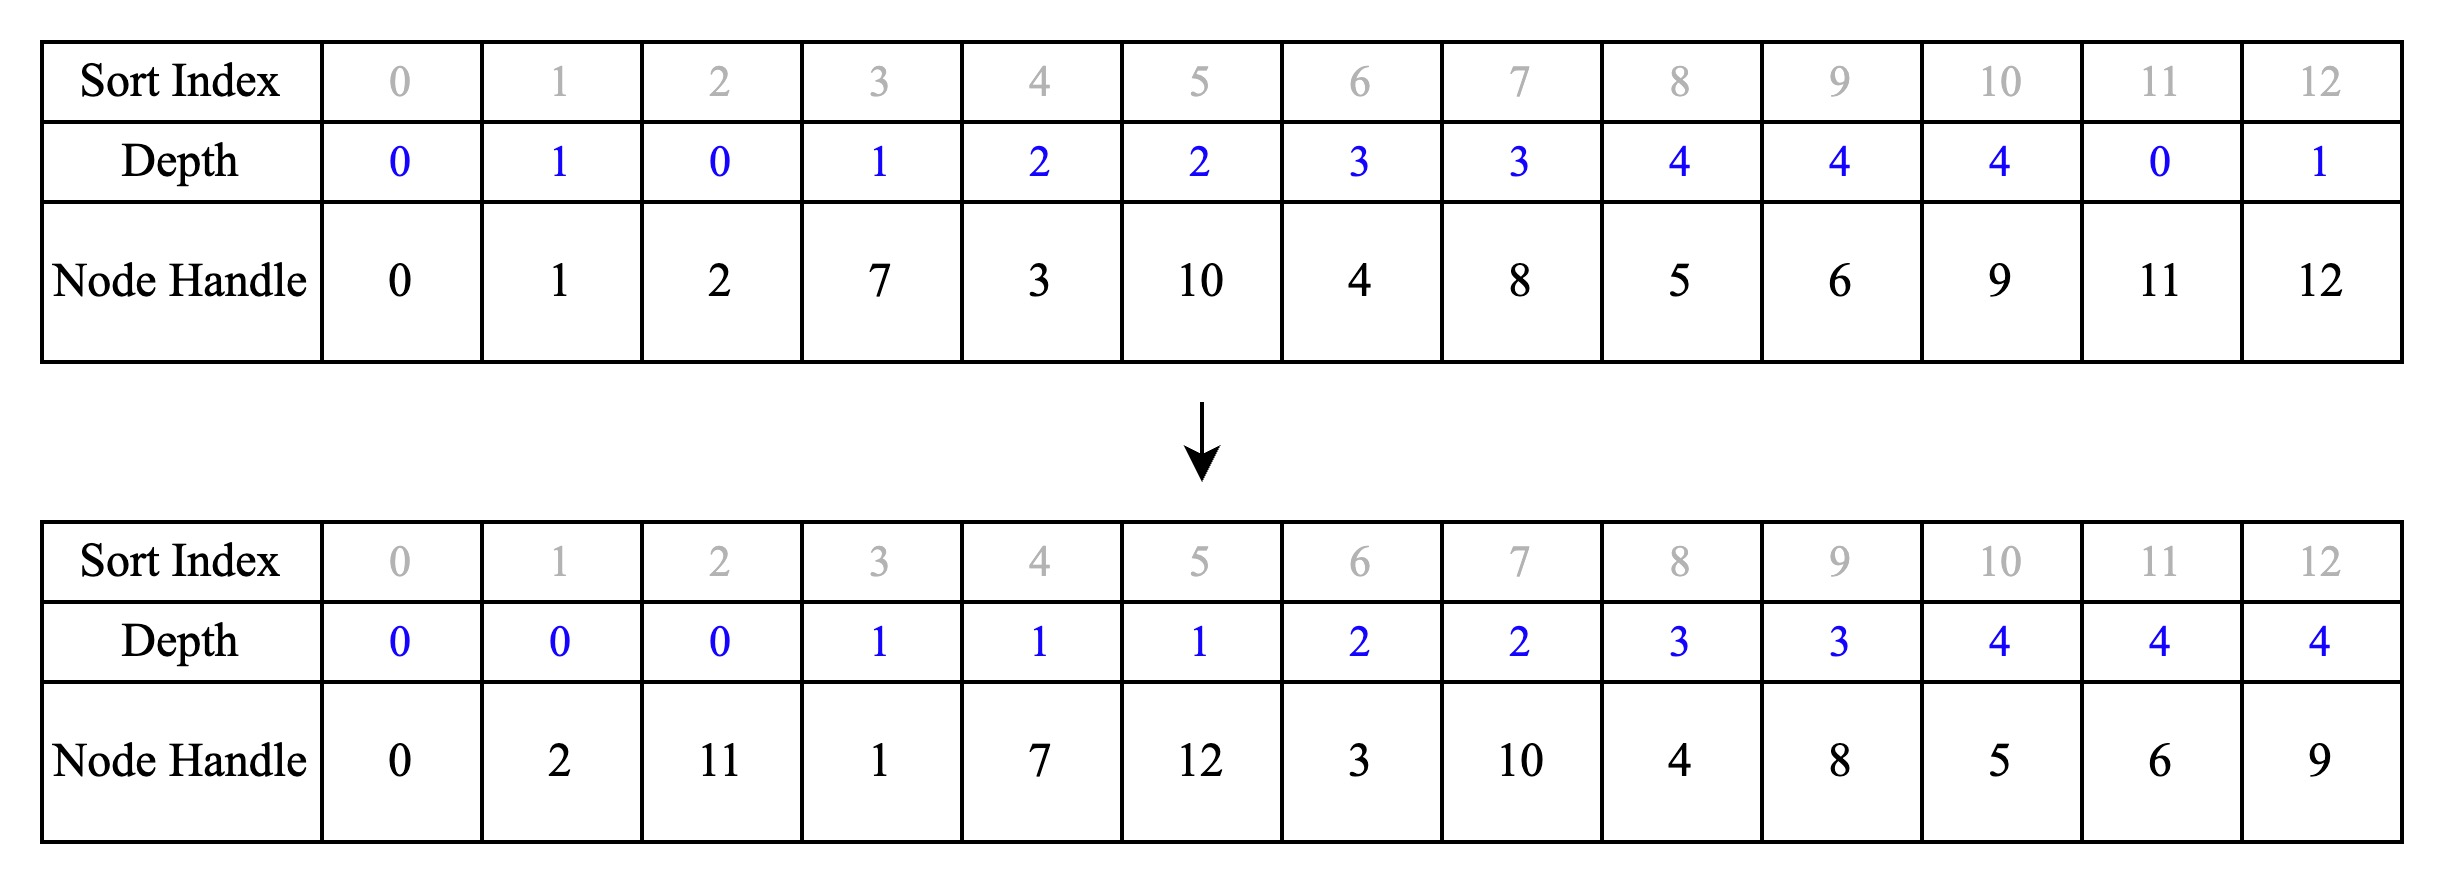
\includegraphics[scale=0.15]{rhi/render_graph/topological_sort_array.jpeg}
    \caption{Первый массив -- произвольная топологическая сортировка, второй -- перестановка первого, упорядочивающая глубину по неубыванию (оставаясь при этом топологической сортировкой).}
    \label{fig:render_graph_topological_sort_arrays}
\end{figure}

\subsubsection{Отсечение ребер}
Теперь избавимся от ненужных ребер графа для дальнейшего определения точек синхронизации командных очередей. Этот этап критически важен для оптимизации работы графа и уменьшения накладных расходов на синхронизацию. Данная часть алгоритма основана на статье \cite{organizing_gpu_work_with_directed_acyclic_graphs} и идентична для всех современных графических API. Предположим, у нас есть $Q$ командных очередей. Также для каждой вершины нам известен индекс очереди, на которой она будет исполняться -- $queue\_idx(u) \in \{0,...,Q-1\}$. Прежде всего необходимо переиндексировать вершины так, чтобы внутри каждой очереди вершины шли по возрастанию, и для любой пары очередей $q_1, q_2 \in \{0,...,Q-1\}$, таких что $q_1 < q_2$, все вершины очереди $q_1$ имели индексы меньше, чем индексы всех вершин очереди $q_2$. Положим в качестве такой переиндекцации $\sigma(u) = sort\_idx(u) + queue\_idx(u) \cdot V + 1$. Также для каждой вершины введем так называемый \textit{Sufficient Synchronization Index Set} (сокращенно \textit{SSIS}), для каждой очереди показывающий индекс $\sigma$ вершины, с которой достаточно синхронизировать данную вершину. Формальное определение \textit{SSIS} представлено в равенстве \ref{eq:ssis_definition}. Граф с посчитанными \textit{SSIS} можно увидеть на рисунке \ref{fig:cross_queue_graph_original}.

\begin{align}
    i_{q}(u) &= \left\{ \begin{array}{rcl}
        \sigma(u) & \mbox{если} & q = queue\_idx(u) \\
        0 & \mbox{иначе, если} & \forall v: (u, v) \notin E(G^R) \\
        \underset{d(v) \leq d(u)}{\underset{(u,v) \in E(G^R)}{\arg\max}} \{\sigma(v)\} & \mbox{иначе}
    \end{array}\right.&\\
    SSIS(u) &= \left( i_0(u), ..., i_{Q-1}(u) \right) \label{eq:ssis_definition}
\end{align}

Строить новый граф без лишних ребер (назовем его $G^*$) будем итеративно. Для начала для каждой вершины посчитаем бинарный кортеж $cover$ из $Q$ элементов, каждый элемент которого показывает синхронизирована ли уже данная вершина с данной очередью. Дальше будем в цикле пытаться улучшить ситуацию, пока для всех вершин $cover$ не станет полностью из единиц. На каждой итерации раскрываются все вершины $u$, чьи $cover$ имеют нули. Раскрытие вершины $u$ происходит следующим образом: рассматриваются все вершины $v$, в которые идут ребра реверс графа из $u$, считается промежуточный $cover$ между только этими двумя вершинами, и если данное ребро улучшает глобальный $final\_cover(u)$, то мы запоминаем вершину $v$. Выбрав из всех таких $v$ наилучшую (по количеству единиц, которое она добавляет в $final\_cover(u)$), мы обновляем $final\_cover(u)$ и добавляем в граф $G^*$ ребро $(u, v)$. Полный алгоритм представлен в листинге \ref{lst:render_graph_cross_queue_graph}, а также первая итерация алгоритма проиллюстрирована на рисунке \ref{fig:cross_queue_graph_first_iteration}.
\begin{figure}[htp]
    \begin{subfigure}
        \centering
        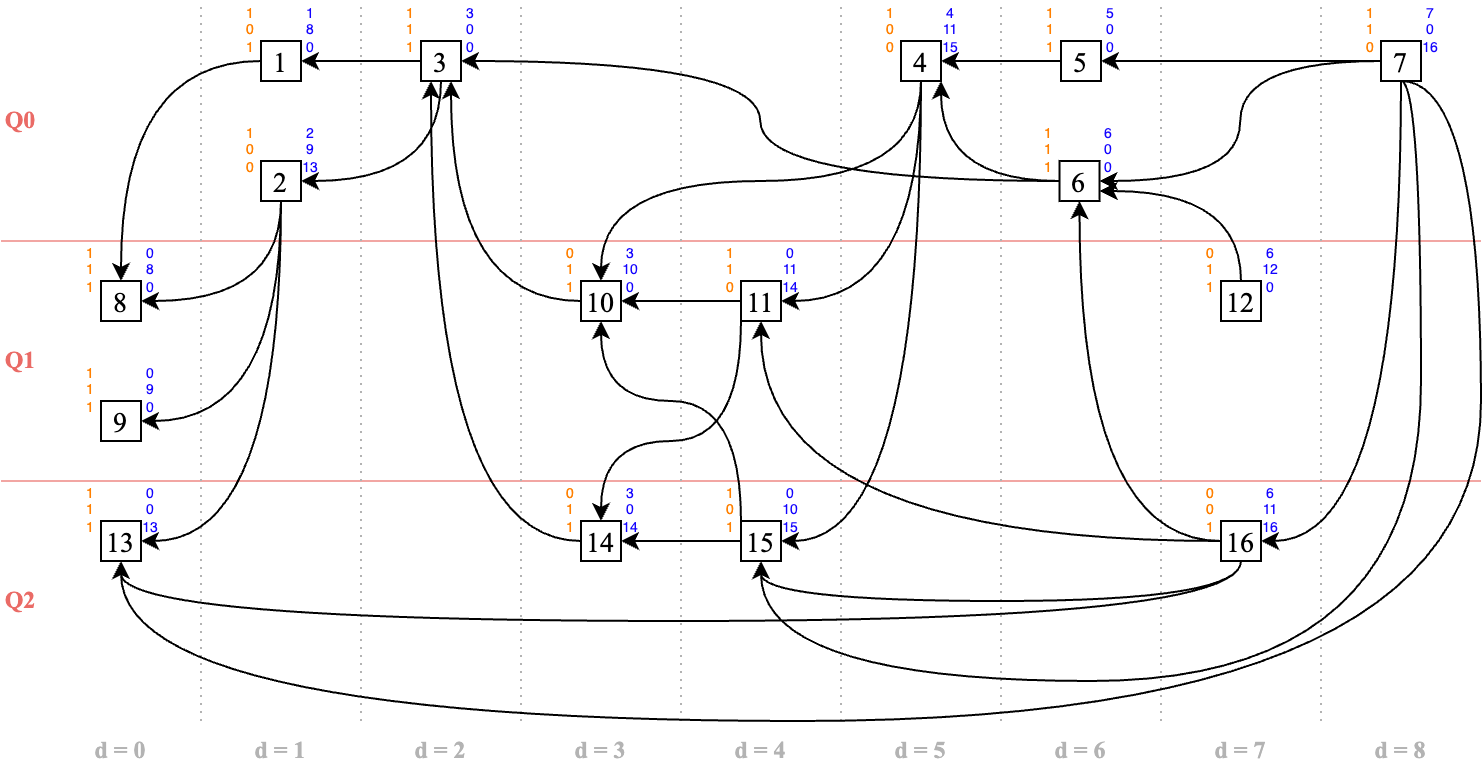
\includegraphics[scale=0.315]{rhi/render_graph/cross_queue_graph_original.png}
        \caption{Изначальный реверс граф, где у каждой вершины справа синим светом подписан $SSIS$, слева оранжевым $final\_cover$, а индексация вершин показывает $\sigma(u)$.}
        \label{fig:cross_queue_graph_original}
    \end{subfigure}
    \bigskip
    \bigskip
    \begin{subfigure}
        \centering
        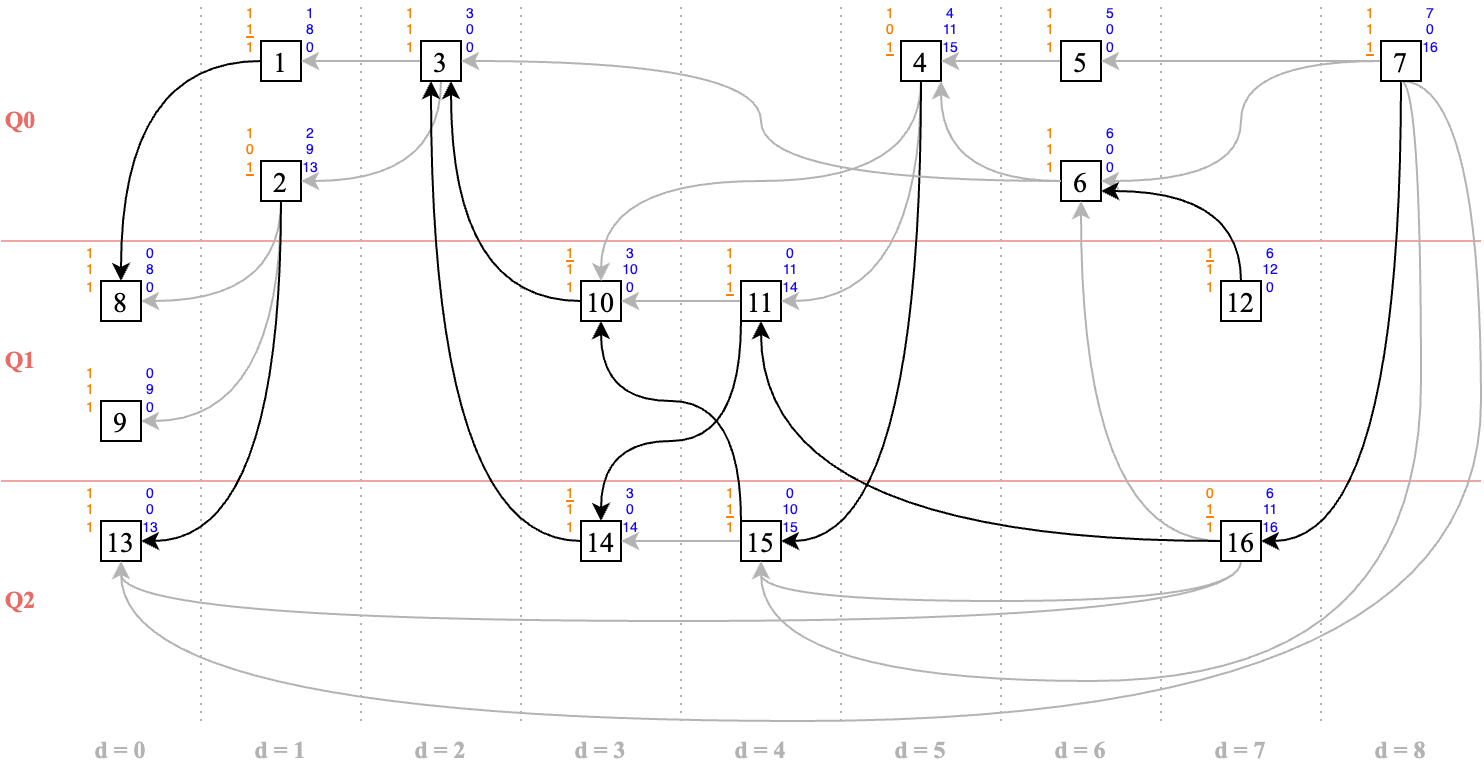
\includegraphics[scale=0.315]{rhi/render_graph/cross_queue_graph_first_iteration.png}
        \caption{Первая итерация алгоритма построения $G^*$.}
        \label{fig:cross_queue_graph_first_iteration}
    \end{subfigure}
\end{figure}

\begin{minipage}[t]{0.95\textwidth}
    \centering
    \begin{pseudocode}[mathescape=true, caption={Построение графа $G^*$ с достаточным минимальным набором ребер для межочередной синхронизации}, label={lst:render_graph_cross_queue_graph}]

    function CoverScore($cover$):
        return $\sum_{q=0}^{Q-1} cover_q$

    $\forall u: final\_cover(u) \leftarrow (1, ..., 1)$
    $\forall u \forall q \in\{0, ..., Q-1\}: (\exists v: (u, v) \in E(G^R)) \implies final\_cover_q(u) \leftarrow 0$

    $covered\_all$ $\leftarrow$ false
    while not $covered\_all$:
        $covered\_all$ $\leftarrow$ true
        for $u \in G^R$:
            $v^* \leftarrow \emptyset$
            $cover^* \leftarrow final\_cover(u)$
            for $v \in G^R, (u, v) \in E(G^R)$:
                $cover \leftarrow (..., SSIS_q(u) \leq SSIS_q(v), ...)$
                if CoverScore($cover$) $>$ CoverScore($cover^*$):
                    $v^* \leftarrow v$
                    $cover^* \leftarrow cover$
                else if CoverScore($cover$) $=$ CoverScore($cover^*$) and $\sigma(v) > \sigma(v^*)$
                    $v^* \leftarrow v$
                    $cover^* \leftarrow cover$
            if $v^* \neq \emptyset$:
                $final\_cover(u) \leftarrow final\_cover(u) | cover^*$
                $G^* \leftarrow G^* \cup (u, v^*)$
            if CoverScore($final\_cover(u)$) $\neq Q$:
                $covered\_all$ $\leftarrow$ false
    \end{pseudocode}
\end{minipage}

\subsubsection{Синхронизация}
Дальше идет часть компиляции, во многом уникальная для Vulkan. Нам необходимо расставить сабмиты, а также синхронизацию между ними при помощи семафоров (примитивов синхронизации командных очередей). В новых версиях Vulkan появились так называемые \textit{timeline semaphores} (временные семафоры) \cite{vulkan_timeline_semaphore}, способные хранить 64-битное число вместо бинарного флага. Поэтому в данной работе предлагается использовать именно их, ввиду их гибкости и сильного снижения количества необходимых примитивов синхронизации.

Сабмиты ставятся в конце каждой командной очереди, а также после каждого уровня глубины, на котором существует хотя бы одна вершина, в которую есть входящие ребра графа $G^*$. Такой подход гарантирует необходимую синхронизацию и при этом не влечет излишних задержек. На каждую командную очередь выделяется по одному временному семафору. Поскольку значения должны монотонно возрастать, каждое значение можно представить как $$Timepoint(frame\_idx, submit\_idx) = frame\_idx \cdot V + submit\_idx \text{.}$$
В данном определении $V$ -- произвольное число, заведомо большее числа сабмитов на каждой очереди, а $submit\_idx$ -- индекс сабмита на конкретной очереди в 1-индексации. Дальше достаточно на основе ребер $G^*$ расставить значения ожидания/сигнала на каждом сабмите. Финальную версию графа $G^*$ с выставленными сабмитами можно увидеть на диаграмме \ref{fig:cross_queue_graph_submits}.

Немаловажной частью работы с Vulkan также является ручная расстановка барьеров исполнения для ресурсов. Правильная расстановка барьеров критична для предотвращения ошибок гонки данных. Если ресурс используется исключительно в одной очереди, то автоматическая расстановка барьеров в таком случае тривиальна, хотя и требует внимательного рассмотрения всех параметров. Сложность возникает, когда ресурс используется на нескольких очередях. Самый простой вариант решения данной проблемы -- это создание всех ресурсов с указанием автоматического кросс-очередного использования. Однако этот подход может повлиять на производительность, например, делая невозможным использование \textit{delta color compression} \cite{optimising_a_aaa_vulkan_title_on_desktop}. Второй же подход -- расставлять барьеры с \textit{queue ownership transfer}. В целом, в текущей имплементации графа расстановка данных барьеров не требует больших усилий, поэтому этот подход более предпочтительный.

\begin{figure}[h]
    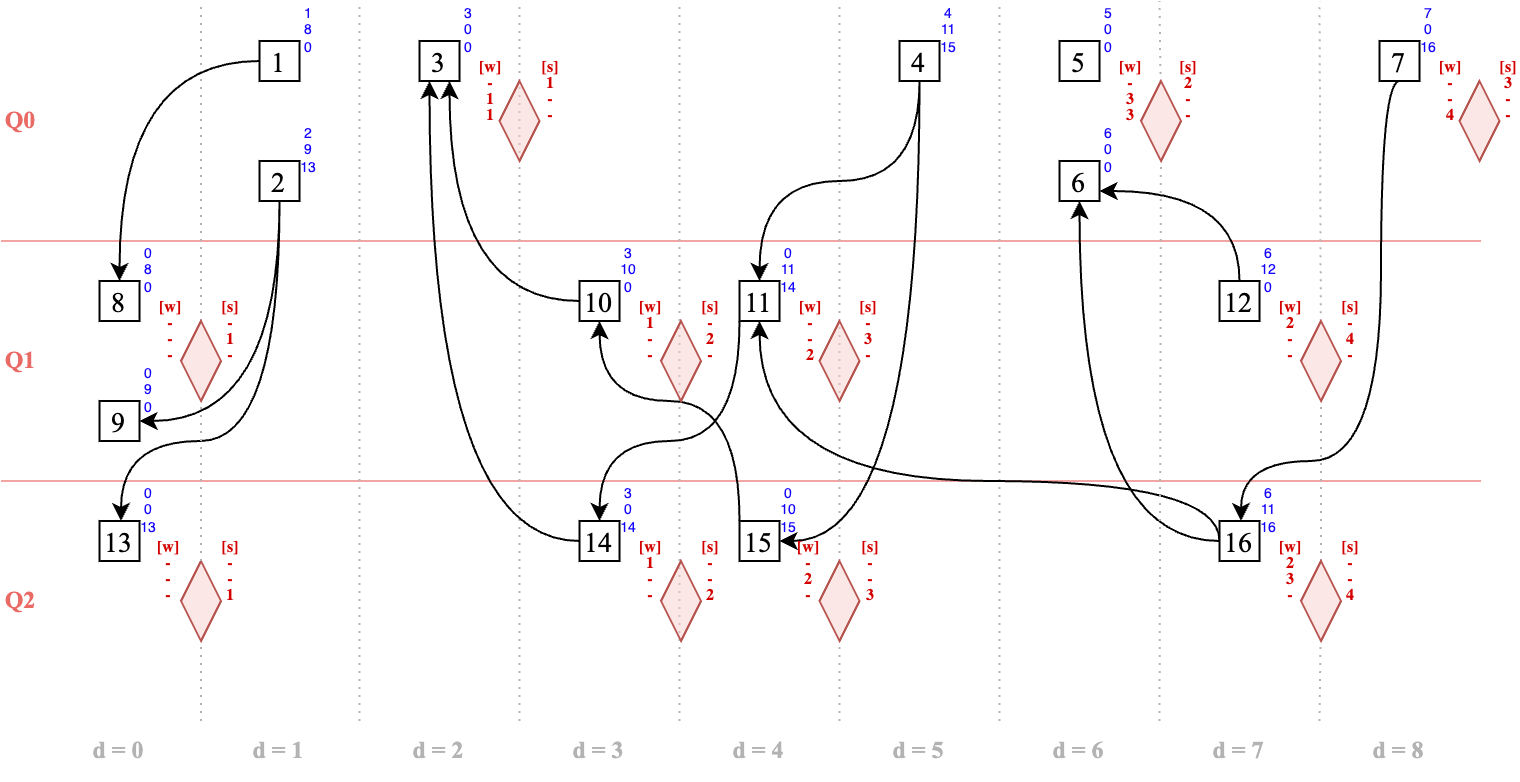
\includegraphics[scale=0.308]{rhi/render_graph/cross_queue_graph_submits.png}
    \caption{Финальный граф $G^*$ с выставленными сабмитами. Слева от каждого сабмита подписаны значения для ожидания на каждую очередь, а справа -- значения для сигнала.}
    \label{fig:cross_queue_graph_submits}
\end{figure}

\subsection{Отладочная информация}
Для отладки были разработаны два вида визуализации конкретных кадровых графов с помощью инструмента Graphviz \cite{graphviz} -- краткая и подробная. Краткая версия предоставляет общую картину графа, что помогает быстро определить корректность "потока" ресурсов в графе. Подробная же отображает дополнительно все параметры ресурсов, типы их использования, а также барьеры. Эта информация особенно полезна при выявлении узких мест и оптимизации производительности рендеринга. Дополнительно, проставляются имена ресурсов и вершин, а также именные границы команд в командных буферов по тому, какой вершине они принадлежат, с помощью специального расширения для Vulkan -- VK\_EXT\_debug\_utils \cite{vulkan_ext_debug_utils}. Данная информация помогает при графической отладке в приложениях, таких как RenderDoc \cite{renderdoc}. Пример показан на рисунке \ref{fig:renderdoc_capture_debug_utils}. Представленные механизмы позволяют легко идентифицировать причины ошибок и конфликтующие зависимости между ресурсами, что значительно ускоряет процесс разработки.

\begin{figure}[h]
    \centering
    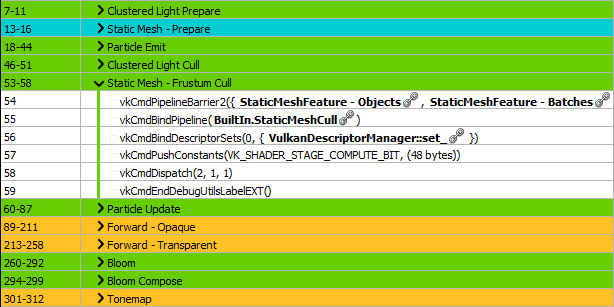
\includegraphics[scale=0.7]{rhi/renderdoc_capture_debug_utils.jpg}
    \caption{Скриншот из RenderDoc, показывающий этапы встроенного рендерера (синий цвет означает transfer, зеленый означает compute и оранжевый -- graphics), а также отображающий имена ресурсов (см. события 54-56).}
    \label{fig:renderdoc_capture_debug_utils}
\end{figure}

\subsection{Структура кадра}
В отличие от оригинального решения, предложенного в \cite{frame_graph_frostbite}, в данной работе была реализована возможность наличия нескольких кадровых графов. Существует два способа исполнения графов -- последовательное и асинхронное. Последовательное исполнение синхронизируется при помощи временных семафоров, аналогично механизму синхронизации сабмитов, разобранному в пункте про компиляцию графов. В данном случае формула момента времени становится $$Timepoint(frame\_idx, graph\_idx) = frame\_idx \cdot G + graph\_idx\text{,}$$где $G$ -- произвольное число, заведомо большее числа графов на кадр. При асинхронном же исполнении синхронизации не происходит. Завершение асинхронного исполнения можно проверить вручную, либо же указав callback при отправке графа на исполнение. Возможность наличия нескольких кадровых графов позволяет более гранулярно разбить разные модули игрового движка, занимающиеся работой с GPU. Так, например, на рисунке \ref{fig:several_render_graphs} представлено возможное разбиение работы на: рендеринг игры, рендеринг в инструментах редактора, отрисовка пользовательского интерфейса, а также асинхронный трансфер данных и генерация preview изображений для редактора. Такой подход позволяет легко масштабировать систему, добавляя новые графы для концептуально новых задач без изменений в уже существующих. Использование нескольких кадровых графов также обеспечивает изоляцию между различными подсистемами, что повышает стабильность и упрощает отладку.

\begin{figure}[h]
    \centering
    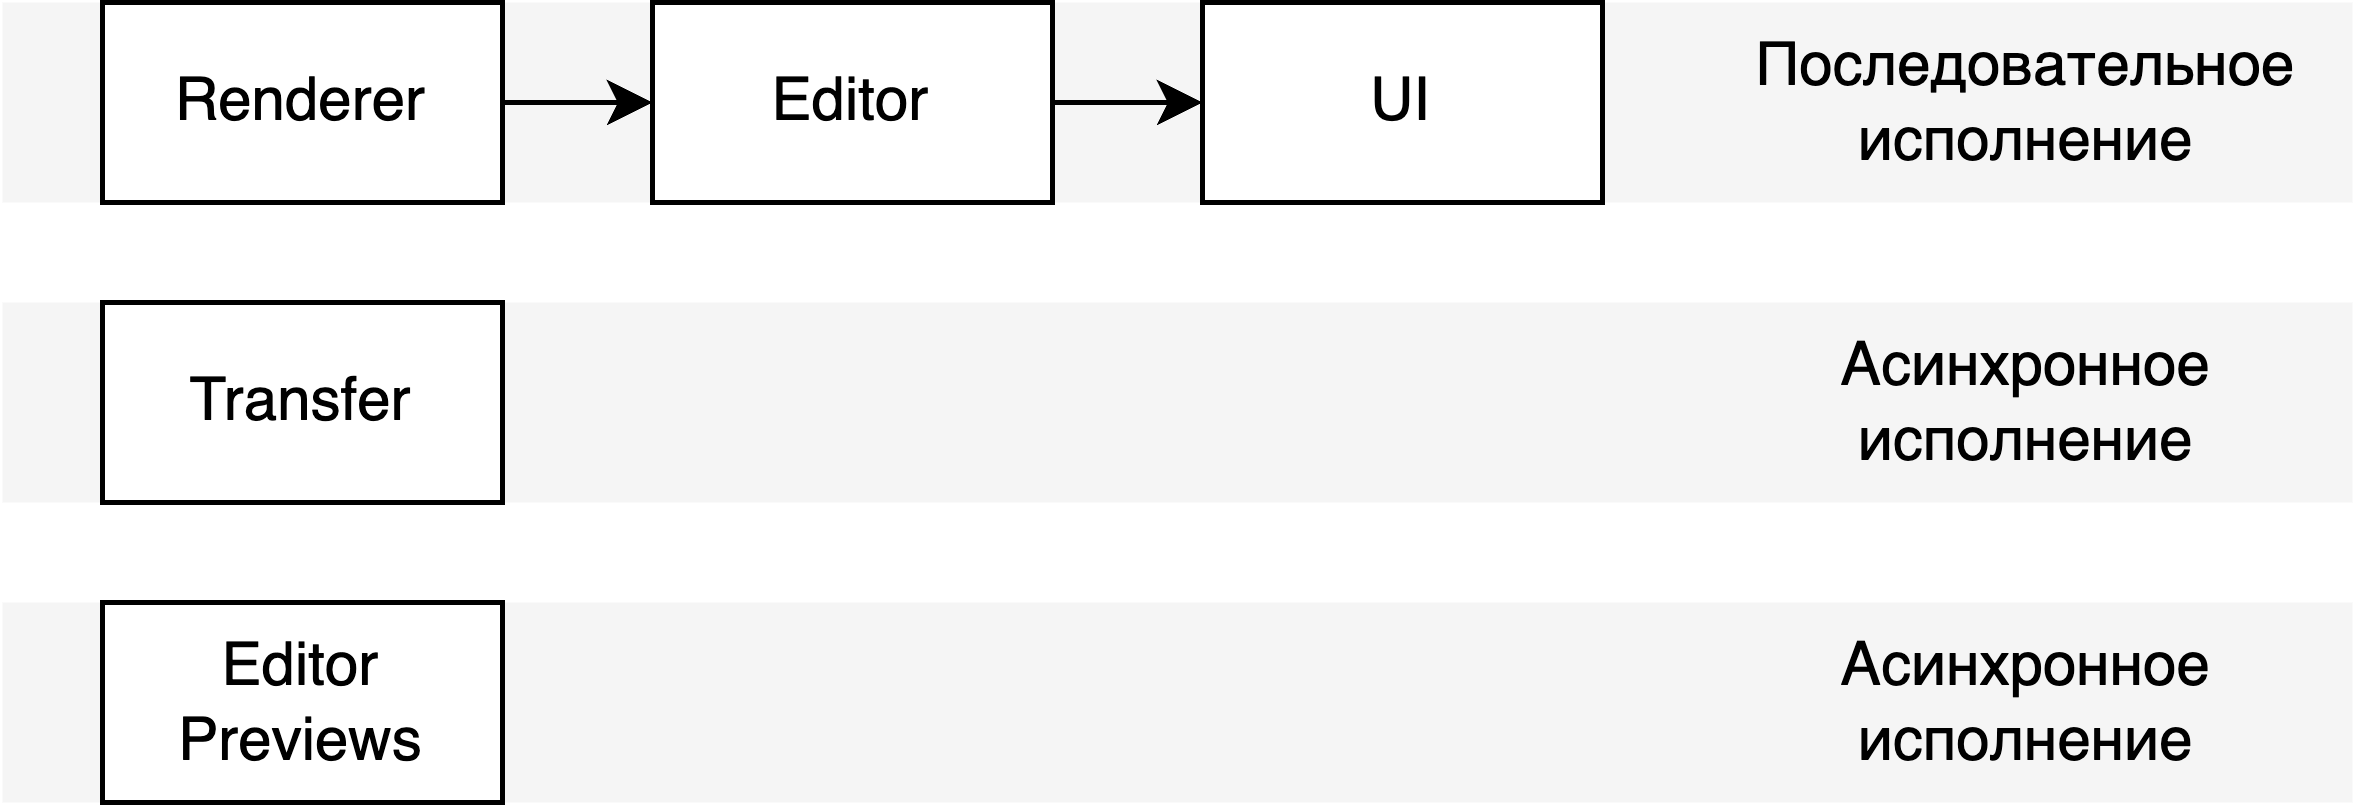
\includegraphics[scale=0.15]{rhi/render_graph/several_render_graphs.png}
    \caption{Виды композиции исполнения кадровых графов и примеры использования данной функции.}
    \label{fig:several_render_graphs}
\end{figure}